\chapter{As Partes Interessadas na Sua Tese}

\begin{center}
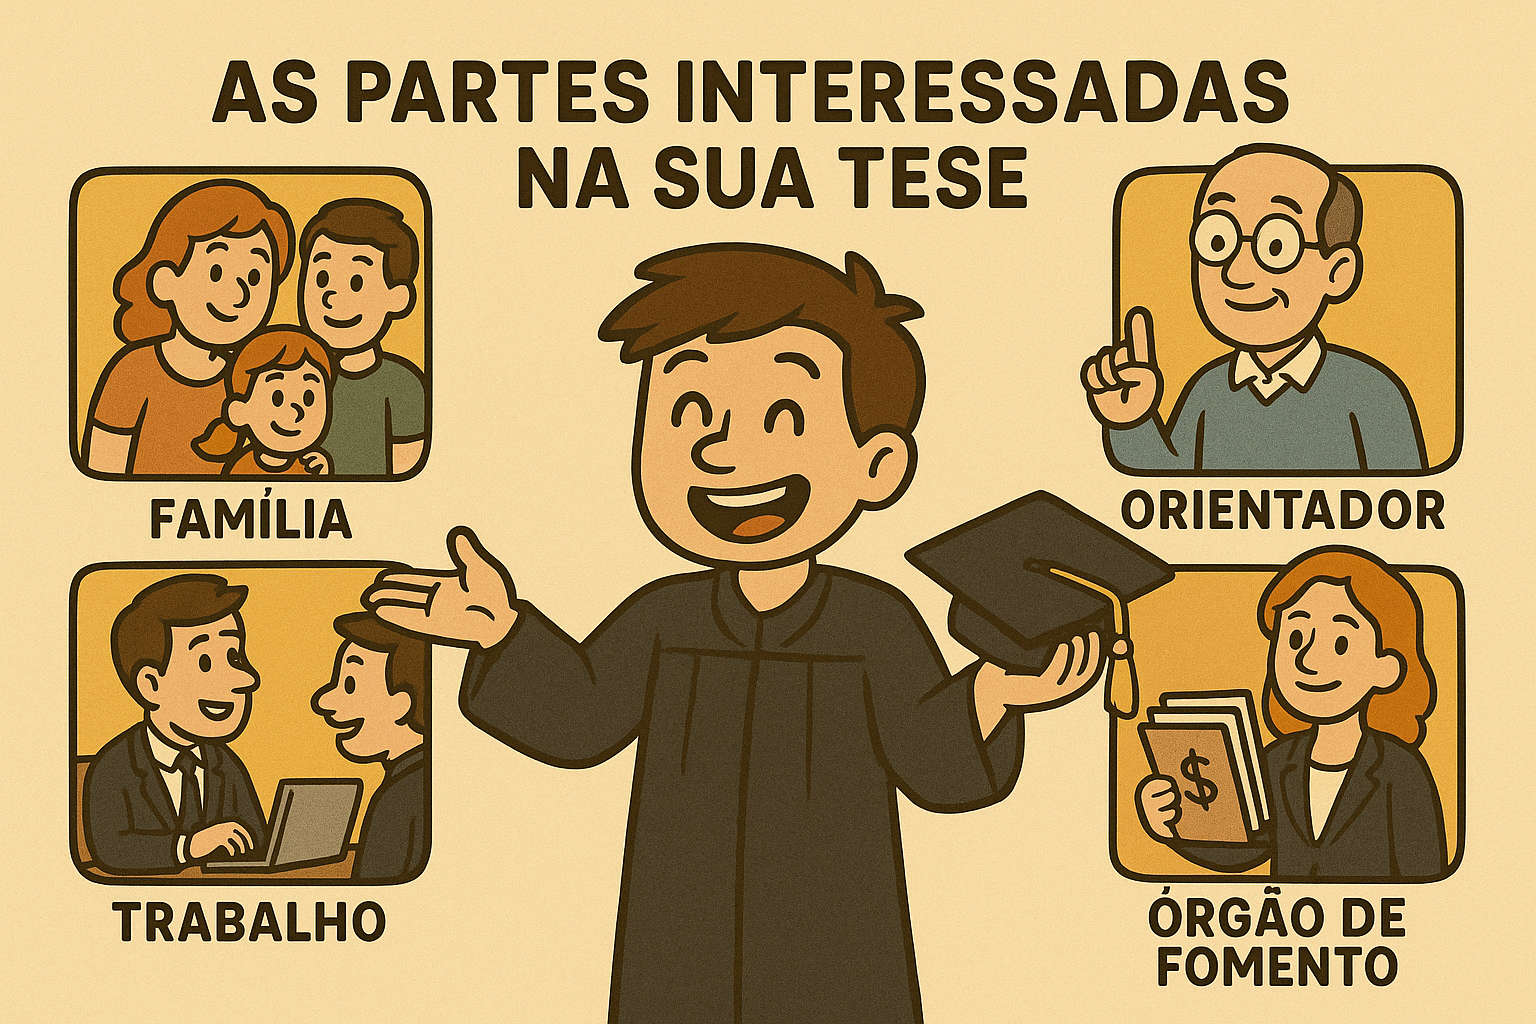
\includegraphics[width=0.5\linewidth]{Images/partesinteressadas.png}    
\end{center}
\vspace{0.5cm}

Toda tese é um projeto. As boas práticas de projeto sugerem que você levante, no início do projeto, e controle e gerencie, ao longo do projeto, as partes interessadas no projeto.
Mas o que são as partes interessadas? Não seriam apenas você, ou você e seu orientador, as únicas partes interessadas?

Uma parte interessada é qualquer pessoa ou grupo que afete ou seja afetado pela sua tese, de verdade ou por percepção. A partir dessa definição, vemos que existem muito mais partes interessadas.

Por exemplo, todos que se relacionam de maneira afetiva no dia a dia com você serão afetados pela sua tese, e alguns afetarão. 
Sua disponibilidade de tempo e atenção passará a ser dividida com a tese. 
Vários momentos que antes eram livres passarão a ser ocupados com pesquisas, leituras, programação, experimentos e outras atividades. 
Isso pode afetar os seus relacionamentos e você deve prestar atenção para que não prejudique fortemente sua vida pessoal.

Gostaria de contar o caso de um doutorando que mantinha um escritório fechado, para evitar que fosse desorganizado. 
Seu filho pequeno, ao ver a porta aberta, entrou e fez a maior confusão, porque tinha ``raiva'' do pai ficar no escritório e não com ele. Em outro exemplo, um mestre recém-formado ouviu um ultimato de sua esposa: ``Se você for fazer doutorado eu peço o divórcio''. Ele é doutor hoje em dia, e está feliz no segundo casamento.

O \textbf{principal interessado normalmente é você}. Mas não apenas o você científico ou profissional, mas o você ``completo''. Não só você afeta a tese, pois o sucesso dela depende do seu esforço, mas será também afetado por ela. O stress da pesquisa, da defesa, da dívida constante de trabalho, já causou problemas de saúde, física e mental, para muitos. Estudos mostram alarmantes  graus de depressão entre alunos de pós-graduação~\citep{walker2015}.

O \textbf{orientador é outra parte interessada óbvia}. Todo orientador realmente quer que todos orientados defendam sua tese. Porém, são também guardiões da qualidade do diploma, logo, querem que a tese seja boa. Um bom orientador deve reprovar um aluno que não alcance os padrões acadêmicos de sua instituição, mas isso sempre é feito com desgosto. Mais de uma vez compartilhei com colegas a sensação de tristeza de ter um aluno que prometia resultados, mas não consegue, por um motivo ou outro, atingir um padrão de qualidade que garanta sua defesa.

Os membros da banca darão a palavra final da aprovação da sua tese. A tese deve atender a padrões de qualidade, de honestidade científica, e eles são a barreira final. Muitas vezes, seu orientador sinalizará: você precisa atender aos padrões da banca, tem que ser capaz de convencer o leitor.

Depois desses grupos básicos, temos outras partes interessadas. Seu programa, os órgãos de fomento, a universidade, a sua comunidade científica e a sociedade em geral. Todos eles devem ser atendidos. 

Cabe então, a você, ao iniciar sua tese, pensar em como vai atender a todos. Seu orientador pode ajudar.

\section{Sua Família}
Família e tese são quase tão incompatíveis como trabalho e tese. A tese exige atenção. Nem sempre esposa, marido, filhos e filhas estão preparados para perder parte do tempo da atenção que lhes é normalmente dispensada para uma atividade intrinsecamente solitária.

A primeira coisa a lembrar é que você precisa também dar atenção à família. Se decidir estudar todo domingo, por exemplo, saia com as crianças de manhã cedo e só depois comece a estudar. 

Aproveite os momentos de descanso para fazê-los com sua família. 

Antes de começar uma tese, converse com sua família. Explique a necessidade de tempo, apoio e compreensão. Se necessário, deixe acordado desde o início que espaço de tempo será ``integral'' da família e não pode ser tocado. 

A hora de dormir com as crianças, o dever de casa, o cinema no sábado, o jantar romântico, tudo pode ter seu lugar se houver alguma organização de sua parte. 

\section{Seu Trabalho}

Se você trabalha, está em desvantagem. 
Em primeiro lugar, a pós-graduação não foi pensada, principalmente no Brasil, para quem trabalha, mas sim para quem se dedica exclusivamente a pesquisa. 

Além disso, mesmo que seu empregador ou seu chefe tenha prometido a liberação, deixá-lo realizar seu sonho, ele realmente precisa que você trabalhe e ganhe dinheiro para a empresa. Isso significa que todas as promessas do seu empregador serão esquecidas com o tempo.

Algumas organizações, principalmente as públicas, liberam você para fazer sua tese. Para sermos justos, uma liberação de 4 anos, 2 para o mestrado, atende às necessidades de qualquer aluno (mesmo que você tenha mais prazo). É vital acabar a tese antes do final da liberação. Voltar para o trabalho sem terminar a tese não só atrapalha o fim dela como pode ser considerado por seus colegas como uma espécie de ``derrota'', atrapalhando sua carreira. A pior situação possível seria você voltar e nunca acabar a tese! 

Também é comum que o aluno seja liberado para as cadeiras, mas não para o desenvolvimento da tese. Isso é um mau sinal. Caso seja liberado para as cadeiras apenas, tente pelo menos que o tempo de estudo seja incluído nessa liberação. Normalmente, aconselhamos o aluno a considerar que o tempo de estudo para uma cadeira é, no mínimo, duas vezes maior que o tempo de aula. Isso significa que, para cada hora de aula, você teria que ter mais duas horas liberadas, totalizando três horas! Você pode colocar algumas dessas horas de estudo a noite ou no fim de semana, mas não todas.

É importante que você tenha por escrito todas as promessas da companhia, assinadas por uma pessoa com autoridade sobre seu chefe imediato, pelo Diretor de Recursos Humanos ou pessoa comparável.
Se você pertence a uma instituição com atenção curta, que toda hora muda de foco, seus problemas serão maiores. Quanto menor a sua empresa, maiores serão seus problemas. Se seu cargo envolve viagens constantes, seus problemas serão tão grandes que talvez seja impossível você realizar seus cursos ou defender a sua tese.

Se você trabalha na Universidade, então certamente terá mais chances e muito menos problemas. Se você pretende arranjar bicos durante o curso, procure trabalhos ligados à educação.Lembre que, a princípio, investimento na pós-graduação tem muito mais valor que o salário que você deixa de ganhar. 

\section{Os Órgãos de Fomento}

Se você ganha uma bolsa de algum órgão de fomento, como FAPERJ, CAPES e CNPq, você tem a responsabilidade legal de acabar a tese. 
Apesar de não ter sido a prática por muito tempo, atualmente há investigações e pedidos de restituição dos valores pagos como bolsa para alunos que não terminaram suas teses e não possuem uma justificativa.

Atenção também à taxa de bancada. Ela não é um adicional à tese, mas uma verba destinada a gastos na sua pesquisa e que devem ser comprovados. Você terá que prestar um relatório final e pode ser auditado.




